\documentclass[11pt]{article}
\usepackage[margin=1in]{geometry}
% arXiv는 pdfLaTeX로 컴파일한다 (XeLaTeX 비공식). 로컬 Tectonic은 XeLaTeX. 엔진에 따라 나눈다.
\usepackage{iftex}
\ifPDFTeX
  \usepackage[utf8]{inputenc}
  \usepackage[T1]{fontenc}
  \usepackage{lmodern}
  \usepackage{textcomp}
\else
  \usepackage{fontspec}
\fi
\usepackage{newunicodechar}
\usepackage{amsmath,amssymb}
\usepackage{graphicx}
\usepackage{booktabs,tabularx}
\usepackage[round]{natbib}
\usepackage[hidelinks]{hyperref}
\usepackage{caption}
\captionsetup{font=small}
% 본문의 유니코드 기호를 그대로 둔다 (수치 대조용). 수식 기호로 찍는다.
\newunicodechar{−}{\ensuremath{-}}
\newunicodechar{→}{\ensuremath{\rightarrow}}
\newunicodechar{ρ}{\ensuremath{\rho}}
\newunicodechar{θ}{\ensuremath{\theta}}
\newunicodechar{‖}{\ensuremath{\Vert}}
\newunicodechar{≥}{\ensuremath{\geq}}
\newunicodechar{×}{\ensuremath{\times}}
\newunicodechar{β}{\ensuremath{\beta}}
\newunicodechar{ε}{\ensuremath{\varepsilon}}
\newcommand{\paramdist}{\ensuremath{\lVert\theta-\theta_0\rVert/\lVert\theta_0\rVert}}
% 저자·소속은 이 파일만 고치면 된다 (md2tex.py는 이 파일이 있으면 덮어쓰지 않음)
\newcommand{\paperauthor}{Hyunwoo Do}
\newcommand{\paperaffil}{Independent Researcher}
\newcommand{\paperemail}{}


\title{Which Model Should Remember? Anchor Choice in Self-Generated Replay for Multi-Stage Continual Pre-Training}
\author{\paperauthor\\ \paperaffil\ifx\paperemail\empty\else\\ \texttt{\paperemail}\fi}
\date{}
\begin{document}
\maketitle





\begin{abstract}

Self-generated replay protects earlier knowledge during continual pre-training without access to the original data: the model writes its own replay text and trains on it alongside new data. In a multi-stage stream, the text can be written by the original model or by any later checkpoint, which we call the replay \emph{anchor}. We continually pre-train Pythia-410M on Korean, Japanese and Russian Wikipedia, then branch into Greek, and vary the anchor and the replay objective, with control arms for the composition of the replay (all generated text vs English prose only). The decision rules for the C-stage experiments were fixed before any C-stage result was seen, with practical margins calibrated on separate B-stage runs. With two trunks per condition, an original-model anchor retained English much better than a latest-checkpoint anchor, and English forgetting decreased monotonically with anchor age; retention of intermediate languages did not follow a monotone pattern. Beyond retention, replay from the original model partially recovered English that the branch starting point had already lost (a 9.4–15.7 point reduction, not a return to the original level). Replaying text sampled from the latest checkpoint with next-token prediction left English worse than both the branch starting point and a budget-matched replay-free control. Training on the same replay text with a token-level KL objective toward the full teacher distribution removed the detectable excess over that control. Probe KL to the original model was more strongly associated with English forgetting than parameter distance (Spearman 0.979 vs 0.754). These are small-scale results (one 410M model, two trunks).


\end{abstract}
\noindent{\small Tags used throughout: \textbf{[pre-specified]} = decision rule fixed in the lab notes before the result was seen; not publicly registered with a timestamp; \textbf{[exploratory]} = comparison declared in advance without a predicted direction; \textbf{[post hoc]} = pattern noticed after seeing results, not tested. All comparisons use two trunks (seeds 42 and 43).}

\section{Introduction}

When a language model is continually pre-trained on new data, it tends to lose what it knew before. Replaying old data reduces this, but the original data are often unavailable. Self-generated replay sidesteps this by letting a model sample text unconditionally and mixing that text into later training. \citet[Eq.~1]{marek2026} show that the expected next-token prediction (NTP) loss on text generated by the base model equals, up to an additive constant (the base model's entropy), the sequence-level forward KL from the base model to the student, so the two have the same gradient in expectation; the NTP gradient, estimated from sampled tokens, has higher variance. By the same argument (our derivation, not a claim of Marek et al.), NTP on replay sampled exactly from a checkpoint $M_j$ would, in expectation, pull the student toward $M_j$; our replay is sampled with top-p truncation, so this holds only approximately in our experiments. Under this view, which checkpoint writes the replay is not a matter of memory decay but a choice of \textbf{anchor}: the model the student is regularized toward.

In a single-stage setting there is only one sensible anchor (the base model). In a multi-stage stream there are several: the original model, the checkpoint after each earlier stage, and the latest checkpoint. Each anchor has seen a different subset of the stream, so each should protect different knowledge. We are not aware of prior work that directly varies the checkpoint provenance or age of the model generating self-generated replay as a controlled variable in multi-stage language-model continual pre-training. Recent work composes data, function, and weight anchors with merged LoRA for long-horizon memorization in continual fine-tuning \citep{zhang2026}, but does not directly vary which checkpoint generates the replay. Our base-anchor results reproduce the main findings of \citet{marek2026} in this setting (self-generated replay reduces forgetting, and a KL objective does better than NTP). \citet[Fig.~9]{marek2026} also show that NTP replay on substitute data can increase forgetting more than plain fine-tuning, while KL replay does not. Our contribution is the extension to multiple stages, where the anchor can be changed; there, an already-degraded latest checkpoint acts like such a mismatched replay source: NTP replay from it increased English forgetting beyond a replay-free control, and the KL objective removed the detectable excess.

We run a study with pre-specified decision rules with Pythia-410M on a three-stage Wikipedia stream (Korean → Japanese → Russian) and a Greek branch stage. We report four findings, each bounded by the scale of the study (one model, two trunks per condition):

\begin{enumerate}
\item \textbf{Anchor choice shifts the trade-off.} An original-model anchor retained English much better than the latest anchor, and English forgetting decreased monotonically with anchor age; the latest anchor retained Korean better, but intermediate-language retention was not monotone in age. Distinct from retention, the original-model anchor also \textbf{partially recovered} English that the branch start $M_3$ had already lost: English forgetting fell below its level at $M_3$ by at least the practical margin in every domain and both trunks (by 9.4–15.7 points), though not back to the original level (§5.1; Fig. 1, 2a, 3; Table 1).
\item \textbf{Latest-anchor NTP replay can amplify existing degradation.} Replaying text sampled from the latest checkpoint left English worse than the branch starting point and than a budget-matched replay-free control (FT-150, which fills the replay slots with repeated Greek blocks) (§5.2; Fig. 2a; Table 2). This is the effect of a mismatched replay source described by \citet[Fig.~9]{marek2026}, here with a degraded checkpoint as the source.
\item \textbf{A soft-target objective on the same text removed the detectable excess.} Replacing NTP on the sampled tokens with a token-level KL toward the teacher's full distribution, on identical replay text, removed the detectable excess over the replay-free control; hard sampled-target replay is identified as a major contributor to the amplification (§5.3; Fig. 2a; Table 2).
\item \textbf{Output-space distance tracks forgetting.} Probe KL to the original model was more strongly associated with English forgetting than relative parameter distance (§5.4; Fig. 4).
\end{enumerate}


\section{Related Work}

\textbf{Self-generated data and forgetting.} Closest to our work, \citet[\emph{Retaining by Doing}]{chen2026retaining} compare fine-tuning on reward-filtered responses generated once by the initial policy (Self-SFT), which forgets substantially, with regenerating them at the start of every epoch (Iterative-SFT), which forgets little or not at all. Their generated data serve to learn the \emph{new} task; ours serve to \emph{rehearse the old distribution}, and we vary which checkpoint generates it. The direction of the effect also differs: in their setting, new-task data generated by the latest model reduce forgetting, whereas in ours, replay data generated by the latest model can increase it (§5.2). In continual supervised fine-tuning, \citet[\emph{On-Policy Replay}]{chen2026onpolicy} have the latest checkpoint generate responses to a small set of prompts from earlier tasks, filter them by task reward, and replay the surviving (prompt, model response) pairs as ordinary SFT examples, with no teacher and no auxiliary loss. This is close to our latest anchor, in that the latest model writes the replay, but their setting is continual SFT and their responses are conditioned on earlier-task prompts and filtered by reward; ours is pre-training text generated unconditionally from EOS, with no quality filter (only the genre filter of the English-prose arms). They also report that, in their setting, low-scoring replay does worse than vanilla replay, a related observation to our result for unfiltered latest-checkpoint replay (§5.2). The self-synthesized rehearsal (SSR) of \citet{huang2024} likewise has a large language model synthesize its own rehearsal data in place of stored examples. Self-distillation fine-tuning has also been used to recover performance lost to SFT forgetting, quantization and pruning \citep{liu2026}. \citet{zhang2026} study continual supervised fine-tuning over 100 question-answering tasks without storing past training examples, composing data, function and weight anchors with merged LoRA; across three datasets, average final retention rose from 1.2\% to 34.9\%. They do not directly vary which checkpoint generates the replay.

\citet{marek2026} relate NTP on base-generated replay to forward KL toward the base model (Eq. 1): the two have the same gradient in expectation, and the NTP estimate has higher variance. In their Fig. 9, NTP replay on substitute data increased forgetting more than plain fine-tuning, while KL replay did not; we observe the analogous pattern when the replay source is a degraded latest checkpoint in multi-stage continual pre-training (§5.2–5.3). In a toy sequential setting they also regenerate the replay text with the current model before each task, which in effect uses the latest model as the teacher, but they do not vary the teacher. Most of their experiments with real language models involve a single new task, and they list multi-task continual learning as a limitation. Our base-teacher results are consistent with theirs (self-generated replay reduces forgetting; KL does better than NTP; §5.1–5.3). We extend the setting to multiple stages, vary the teacher, and note that with top-p sampling (p = 0.95, as here) the equality of Eq. 1 does not hold, which motivates our KL comparison (§4, C4).

\textbf{Generative replay across stages.} SG-Rep \citep{resta2024} maintains a fixed-size replay memory of synthetic samples generated by the model at each stage of continual machine translation, updated by reservoir sampling. The memory therefore mixes samples of different ages, but age is not studied as a variable. We hold the anchor fixed within an arm and vary its age (§4, C3). In continual learning of diffusion models, generative replay performed worse than naive fine-tuning, and distillation resolved this \citep{masip2025}; our C4 comparison of NTP and KL on the same replay text asks a related question for language models.

\textbf{When and what to replay.} In continual fine-tuning of language models, FOREVER \citep{feng2026} schedules replay of stored examples using a notion of model time defined by optimizer update magnitudes, and its authors note that this is an indirect proxy. Our P5 comparison (§5.4) concerns a related question in a different setting: in our runs, an output-space measure (probe KL) was more strongly associated with forgetting than relative parameter distance. We did not run FOREVER's schedule and make no comparison with it. When to Review \citep{atreya2026} schedules, under a replay budget during continual pre-training, when new examples are trained on as well as when stored examples are replayed; it studies scheduling of real data, not regeneration. \citet{abbes2026}, a closely related study on replay in multilingual continual pre-training, replay stored earlier examples and study replay together with gradient alignment. We do not keep the original data: replay is generated by a model, and the provenance and age of the generating checkpoint are the variables. \citet{fedus2020} study replay capacity, the age of replayed experience (the age of the oldest policy in the buffer) and the replay ratio in reinforcement learning; anchor age is the analogous axis for generated replay in language-model pre-training.

\textbf{Side effects of replay.} \citet{kotha2026} find, in a controlled 150M-parameter setting, that replaying generic pre-training data can also improve data efficiency on the new task; this is why we measure acquisition of the new language separately (Greek, §3.3). \citet{mahdaviyeh2026} show, in over-parameterized continual linear regression, that replay can provably increase forgetting, which connects to our amplification result (§5.2). In continual post-training, \citet{wang2026} find that dense on-policy self-distillation forgets more than GRPO and can collapse, and that a self-reinforcing teacher–student loop can amplify anomalous format patterns. Model collapse \citep{shumailov2024} describes degradation from recursive training on generated data, in which the tails of the original distribution disappear; the amplification we observe shows a similar self-reinforcing dynamic within a single stage, and we do not claim it is the same phenomenon.


\section{Setup}

\subsection{Model, stream and training}
We use Pythia-410M \citep{biderman2023}. The stream is Wikipedia (2023-11-01 dump) in Korean (cycle 1), Japanese (cycle 2) and Russian (cycle 3); branches from the end of cycle 3 ($M_3$) learn Greek. The \textbf{original model} (also called \emph{base}) is Pythia-410M before any continual training. A \textbf{trunk} is one run that starts from the original model and trains through the three cycles in sequence; $M_j$ denotes a trunk's checkpoint at the end of cycle j. Each cycle trains on 3,840 new blocks of 512 tokens (about 2.0M tokens), built by concatenating articles with EOS separators and capping each article at 20 blocks. Every cycle re-initializes AdamW (8-bit), uses a constant learning rate of 1.5e-5 after a 10-step linear warmup, 32 blocks per update, and bf16 mixed precision. With replay, 960 replay blocks are added (20\% of 4,800 blocks, 150 steps); without replay (FT) a cycle has 120 steps, keeping new-data exposure equal. Weights are saved in fp16 at the end of each cycle.

\subsection{Self-generated replay and anchors}
An anchor model samples 512 tokens starting from a single EOS token (unconditional), with temperature 1.0 and top-p 0.95, no top-k, and without stopping at EOS. Generation seeds are recorded in a registry that forbids reusing a seed range for a different replay set, so no branch replays text that its starting checkpoint has already trained on. The one explicit exception is C4, which re-uses the replay text of a sibling NTP arm that the branch start $M_3$ never trained on (§4).

\subsection{Evaluation}
\emph{Original knowledge}: perplexity on English held-out sets (Wikipedia, PG-19 books \citep{rae2020}, C4 web text \citep{raffel2020}; 400 blocks each), reported as \% change from the original model per domain. \emph{Intermediate knowledge}: held-out perplexity of earlier stream languages. \emph{New knowledge}: held-out perplexity of the language being learned. Language held-out sets start after the last training article, keep at most 4 blocks per article, and drop any block whose 13-grams overlap the training data by more than 10\% (a rule fixed before training). We also record \emph{probe KL}, the mean token-level KL(original ‖ checkpoint) on 50 fixed English Wikipedia blocks, and \emph{relative parameter distance} \paramdist{}.

\subsection{Decision rules (fixed before results)}
Each condition is run on two trunks (seeds 42, 43); branch arms are paired within a trunk, trunk-level comparisons are paired by seed. A difference \textbf{meets the practical margin} if both pairs differ in the same direction and the mean difference is at least the practical margin for that metric. Margins were computed from the B-stage fresh trunks only (twice the two-seed range of the same kind of quantity, floor 2.0 percentage points): English Wikipedia 2.0, books 7.27, web 2.0, Korean/Japanese/Russian 2.0, Greek 3.03; for the averaged metrics used at the ends of the C3 age curve, 2.13 (English) and 2.0 (intermediate). B-stage runs calibrate margins; C-stage runs test predictions. Margin definitions and the C3 monotonicity rule were revised before any C-stage result was seen (recorded with reasons in the lab notes).

\emph{C4 categories.} For each English domain, C4-P1 places latest\_kl in category \textbf{A} if it forgets less than latest\_full by at least the margin and its difference from FT-150 does not meet the margin; in category \textbf{C} if it forgets less than latest\_full by at least the margin but still more than FT-150 by at least the margin; and in category \textbf{B} if its improvement over latest\_full does not meet the margin. Forgetting less than FT-150 by at least the margin was not a predicted category and would have been reported separately (A*).

\emph{C3 directional age trend.} Anchor age counts the cycles between the anchor and the branch start (age 0 for $M_3$, age 3 for the original model). The English trend is supported if, in both trunks, Spearman's ρ between anchor age and English forgetting is at most −0.8 (forgetting decreases with age) and the two ends (age 0 vs the original model) differ by at least the margin; the intermediate trend is judged in the same way with ρ at least 0.8 (forgetting increases with age). Judgements are computed by a script (\texttt{c\_check.py}) tested on synthetic results beforehand.


\section{Experiments}

\begin{itemize}
\item \textbf{B (trunks)}: FT (no replay) and \emph{fresh} (at the start of each cycle, generate 960 blocks from the current checkpoint), cycles 1→3, two seeds each. A pre-specified gate at cycle 1 compared fresh against FT on English.
\item \textbf{C1 (base-anchor trunks)}: like fresh, but every cycle's replay is generated by the original model with new seeds.
\item \textbf{C2 (branches from $M_3$)}: from each fresh trunk's $M_3$, learn Greek with a 2×2 of anchor (latest = $M_3$, or base) × composition (all generated text, or only blocks classified as English prose, ``EP''; EP arms generate until 960 blocks pass the filter), plus \textbf{FT-150}, a budget-matched replay-free control: no replay, with the 960 replay slots filled by a random repeat of 960 Greek training blocks, so the training budget is the same. The EP filter is a simple rule: a block counts as English prose if at most 30\% of its letters are non-ASCII, it is not flagged as code (code-symbol density above 6\% or more than 30\% code-like lines), at least 20\% of its words are common English function words, and letters make up at least 60\% of its non-space characters. To keep 960 blocks, the EP arms generated 1,176 (base) and 1,488 (latest) blocks.
\item \textbf{C3 (anchor age)}: branches whose replay comes from $M_2$ (end of cycle 2) or $M_1$ (end of cycle 1), and a 50/50 mix (480 base + 480 latest).
\item \textbf{C4 (objective)}: \emph{latest\_kl} and \emph{base\_kl} re-use exactly the 960 replay blocks of \emph{latest\_full} and \emph{base\_full}. They hold the replay text, data order, update size and learning-rate schedule fixed while changing the replay loss, from NTP on the sampled tokens to the token-level KL(teacher ‖ student) summed over the full vocabulary at each next-token position, with the teacher being the checkpoint that generated the text (verified by weight fingerprint); micro-batching and accumulation are adjusted to fit memory. New-data blocks keep NTP in both. This is a \textbf{matched-data objective comparison}, not a perfect pair: at equal weight, NTP and KL gradients differ in magnitude and direction. We verified with the real data loader that every update contains the same 32 blocks in the same order for NTP (micro-batch 4 × 8 accumulation) and KL (2 × 16), with the same learning-rate schedule, and that both losses average over the same 511 prediction positions per block.
\end{itemize}

Table 1 lists the pre-specified predictions and their outcomes.


\begin{table}[t]
\centering
\small
\caption{Pre-specified predictions and outcomes (two trunks; ``meets margin'' = meets the practical margin of §3.4).}
\label{tab:1}
\begin{tabularx}{\linewidth}{lXX}
\toprule
\textbf{ID} & \textbf{Prediction} & \textbf{Outcome} \\
\midrule
Gate & At cycle 1, fresh forgets English less than FT (per domain) & Passed in all three domains \\
C1-P1 & Base-anchor trunk forgets English less than fresh at cycle 3 & Supported (all three domains) \\
C1-P2 & Fresh retains Korean and Japanese better than base-anchor trunk & Partial (Korean yes; Japanese below margin) \\
P1 & base\_full forgets English less than latest\_full & Supported (all three domains) \\
P2 & latest\_full retains Korean/Japanese/Russian better than base\_full & Mixed (Korean, Russian yes; Japanese opposite) \\
P3 & base\_full's English is lower than at $M_3$ by at least the margin, in each trunk & Supported (all three domains) \\
P4 & Source vs dilution: latest\_ep vs base\_ep & Source effect meets margin; dilution effect below margin \\
P5 & Spearman ρ with English forgetting: probe KL > parameter distance & Pre-specified descriptive comparison: 0.979 vs 0.754 \\
C3 & English monotone in anchor age; intermediate monotone in the opposite direction & Partial: English only \\
C4-P1 & Category A / C / B for latest\_kl vs latest\_full and FT-150 & Category A in all three domains \\
C4-P2 & base\_kl is not worse than base\_full on English by at least the margin & Supported \\
\bottomrule
\end{tabularx}
\end{table}


\section{Results}

\subsection{Anchor choice shifts the trade-off (Fig. 1, 3; Table 1)}
\begin{figure}[t]
\centering
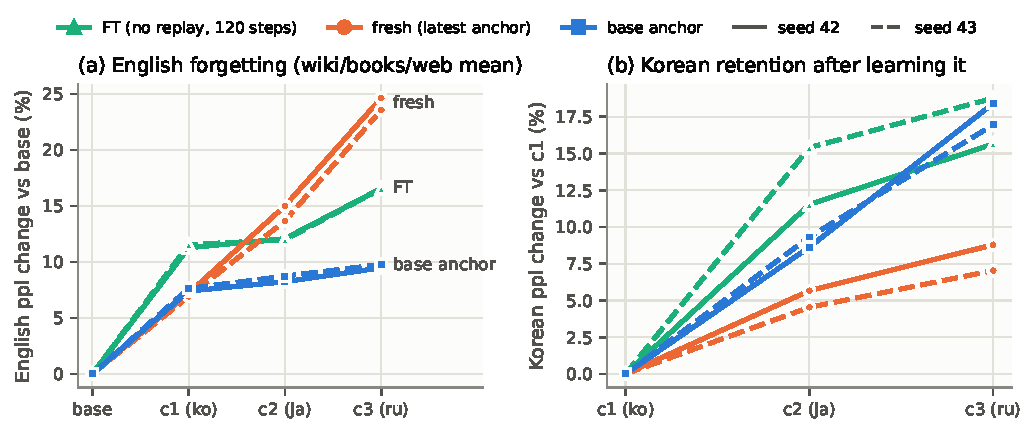
\includegraphics[width=\linewidth]{figures/fig1_trunks.pdf}
\caption{Trunks (B and C1). (a) English perplexity change from the original model (mean of Wikipedia, books and web) after each cycle, for FT (no replay), fresh (latest anchor) and base-anchor trunks; solid and dashed lines are the two seeds. (b) Korean perplexity change relative to the end of cycle 1.}
\label{fig:1}
\end{figure}

\begin{figure}[t]
\centering
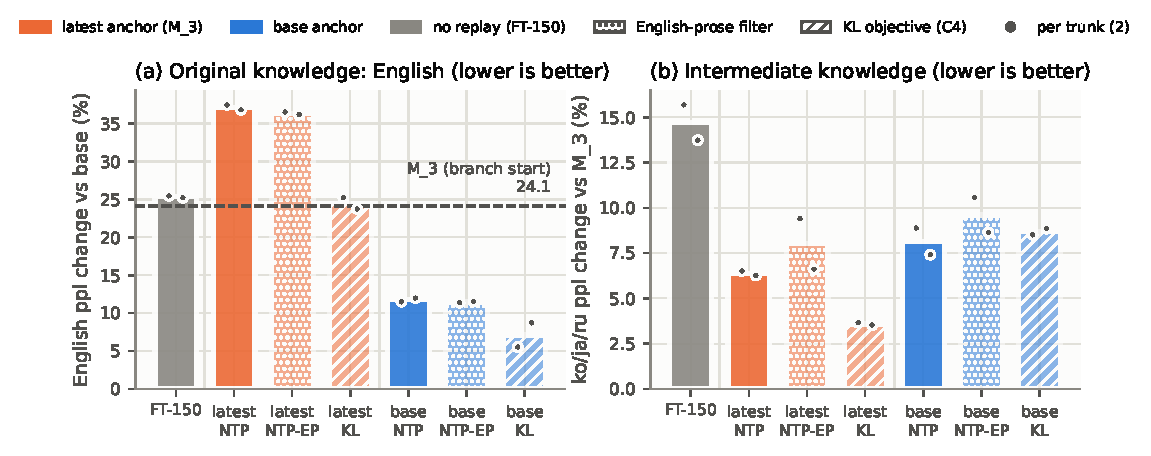
\includegraphics[width=\linewidth]{figures/fig2_branches.pdf}
\caption{Branches from $M_3$ (C2, C4). Bars are the mean of the two trunks, dots the individual trunks. (a) English change from the original model; the dashed line marks the branch start $M_3$. (b) Mean Korean/Japanese/Russian change from $M_3$. Dotted bars: English-prose filtered replay; hatched bars: KL objective on the same replay text as the NTP bar.}
\label{fig:2}
\end{figure}


\textbf{Gate and trunks.} At cycle 1, fresh replay reduced English forgetting relative to FT in every domain (Wikipedia +6.9/+6.3\% vs +10.5/+10.2\%, books +7.3/+6.6\% vs +10.8/+11.8\%, web +7.5/+7.9\% vs +12.6/+12.7\%) \textbf{[pre-specified gate]} (Fig. 1a). Over three cycles, however, the fresh trunks ended with more English forgetting than FT (mean +24.1\% vs +16.6\%) \textbf{[post hoc]}; this comparison is confounded because fresh trains 150 steps per cycle and FT 120 (Fig. 1a).

\textbf{Base vs latest anchor across the stream (C1).} Anchoring every cycle's replay to the original model kept English forgetting at cycle 3 at 8.5–10.2\% across domains and trunks, versus 20.8–27.3\% for fresh (mean differences −12.3, −14.0, −17.1 points) \textbf{[pre-specified, C1-P1 supported]} (Fig. 1a). The latest anchor retained Korean better (increase from cycle 1 to cycle 3: +8.8/+7.0\% vs +18.4/+16.9\%), while the Japanese difference (−1.1 points) was below the margin \textbf{[pre-specified, C1-P2 partial]} (Fig. 1b).

\textbf{Base vs latest anchor at a branch (C2).} From $M_3$, base-anchor replay forgot English far less than latest-anchor replay (−21.5, −23.4, −31.3 points) \textbf{[pre-specified, P1 supported]} (Fig. 2a).

\textbf{Recovery, not only retention (P3).} Retention means losing less during the new stage; recovery means undoing loss that happened before it. The branch start $M_3$ had already lost English (24.6/23.6\% above the original model on average), and learning Greek with base-anchor replay brought English forgetting below its level at $M_3$ by at least the margin in every domain and both trunks: by 9.4 and 9.7 points on Wikipedia, 14.4 and 9.8 on books, and 15.7 and 15.3 on web \textbf{[pre-specified, P3 supported]} (Fig. 2a; Table 2). This is a \textbf{partial recovery}: base\_full still ends 11.5/12.0\% above the original model, so English does not return to the original level. Using self-generated data to recover lost performance has a counterpart in self-distillation fine-tuning after forgetting or compression \citep{liu2026}; here recovery comes from replay generated by the original model during a new stage.

\textbf{Anchor age (C3) and intermediate knowledge.} Across anchors of age 0 to 3 ($M_3$, $M_2$, $M_1$, base), English forgetting decreased monotonically in both trunks (37.5 → 26.3 → 18.5 → 11.5\% and 36.8 → 27.5 → 22.0 → 12.0\%; ρ = −1; ends differ by −25.4 points) \textbf{[pre-specified, C3 English supported]} (Fig. 3a). Intermediate knowledge did not follow the predicted pattern: the latest anchor retained Korean and Russian better than the base anchor, Japanese went the other way (+2.55 points) \textbf{[pre-specified, P2 mixed]}, and the age curve was not monotone (ρ = 0.4 and 0.8; ends differ by 1.76 < 2.0) \textbf{[pre-specified, C3 intermediate not supported]} (Fig. 2b, 3b). The 50/50 mix, which has no single anchor age, fell between the extremes on English (15.5/16.7\%) and was not better than base\_full; H2 was not converted into a pre-specified test, so we report it descriptively (Fig. 3, shown apart from the age axis).

\begin{figure}[t]
\centering
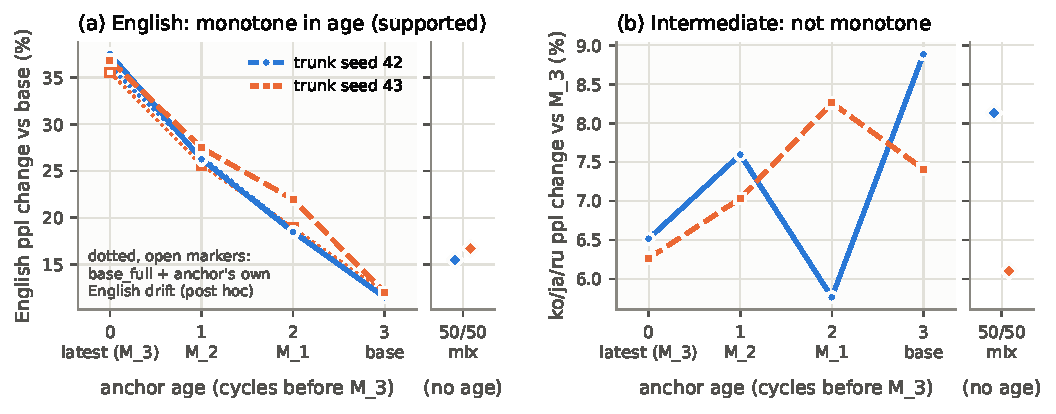
\includegraphics[width=\linewidth]{figures/fig3_age.pdf}
\caption{Anchor age (C3). (a) English change versus the age of the anchor that generated the replay (0 = $M_3$, 3 = original model); dotted lines with open markers show the post hoc description ``base\_full plus the anchor's own English drift''. (b) Intermediate-language change from $M_3$. The 50/50 mix has no single anchor age; it is shown in a separate narrow panel to the right of each age panel, off the age axis.}
\label{fig:3}
\end{figure}


\textbf{A simple description of the English curve [post hoc].} Branch English forgetting is close to ``base\_full's level plus the anchor's own English degradation'': the residuals are −0.2, −0.3 and +1.3 points in trunk 42 and +3.0, +1.8 and +1.3 in trunk 43 for $M_1$, $M_2$ and $M_3$ (dotted lines in Fig. 3a). This relation was fitted after seeing the results and is not a test.

\subsection{Latest-anchor NTP replay can amplify degradation (Fig. 2a; Table 2)}

After learning Greek with replay sampled from $M_3$ (latest\_full), English forgetting was 37.5/36.8\%, higher than at the branch start $M_3$ (24.6/23.6\%) and higher than FT-150 (25.5/25.2\%), which used the same budget without replay (differences to FT-150 meet the practical margin in all three domains) \textbf{[exploratory]} (Fig. 2a; Table 2). Latest-anchor replay can therefore amplify existing degradation rather than only maintain it. This parallels the substitute-data result of \citet[Fig.~9]{marek2026}, where NTP replay increased forgetting more than plain fine-tuning while KL replay did not; here the mismatched replay source is a degraded latest checkpoint in multi-stage continual pre-training (the KL side is in §5.3). Filtering the replay to English prose did not help (latest\_ep 36.5/36.2\%). In the pre-specified 2×2, the source effect (latest\_ep − base\_ep: +21.2, +23.6, +29.9 points) met the practical margin in every domain, while the dilution effect (latest\_full − latest\_ep: +0.34, +0.08, +1.98) was below the margin in every domain \textbf{[pre-specified, P4: source effect meets margin; dilution effect below margin]}. This is consistent with a self-reinforcing dynamic similar to model collapse, within a single stage; we do not claim it is the same phenomenon. In the B trunks, the share of non-English blocks in fresh replay grew from 6–10 of 960 at cycle 1 to 113–137 at cycle 3 \textbf{[post hoc]}, but the P4 result indicates that composition alone does not account for the amplification.

Under the same budget, base\_full retained both English (−11.6 to −16.0 points vs FT-150) and intermediate languages (Korean −7.2, Japanese −4.4, Russian −8.0 points) better than FT-150, meeting the practical margin, and no loss in Greek acquisition was detected (difference 0.87 points, margin 3.03) \textbf{[exploratory]} (Fig. 2; Table 2). FT-150 barely changed English relative to $M_3$ (+24.1\% → +25.3\% on average). FT-150 is a no-replay reference under the same conditions; it does not isolate interference from new data perfectly, because the replay slots are filled with repeated Greek blocks.


\begin{table}[t]
\centering
\small
\caption{Branch results (mean of three domains for English; two trunks, 42 / 43). English: \% change from the original model. Intermediate: mean of Korean/Japanese/Russian, \% change from $M_3$. Greek: \% change from $M_3$ (negative = learned).}
\label{tab:2}
\begin{tabular}{llllll}
\toprule
\textbf{Arm} & \textbf{Anchor} & \textbf{Objective} & \textbf{English} & \textbf{Intermediate} & \textbf{Greek} \\
\midrule
$M_3$ (branch start) & – & – & 24.6 / 23.6 & – & – \\
FT-150 & none & – & 25.5 / 25.2 & 15.7 / 13.7 & −35.2 / −30.7 \\
latest\_full & $M_3$ & NTP & 37.5 / 36.8 & 6.5 / 6.3 & −34.7 / −29.0 \\
latest\_ep & $M_3$ & NTP, English prose & 36.5 / 36.2 & 9.4 / 6.6 & −34.4 / −29.4 \\
latest\_kl & $M_3$ & KL & 25.2 / 23.7 & 3.7 / 3.5 & −34.6 / −30.2 \\
base\_full & base & NTP & 11.5 / 12.0 & 8.9 / 7.4 & −34.4 / −29.7 \\
base\_ep & base & NTP, English prose & 11.4 / 11.6 & 10.6 / 8.6 & −34.1 / −29.6 \\
base\_kl & base & KL & 5.5 / 8.7 & 8.5 / 8.9 & −34.3 / −29.4 \\
\bottomrule
\end{tabular}
\end{table}

\subsection{Soft targets on the same text (Fig. 2a; Table 2)}

With the replay text held fixed, switching the replay loss of the latest-anchor arm from NTP to KL reduced English forgetting by 11.3, 10.9 and 15.8 points (meeting the practical margin in all domains), and left no difference from FT-150 that meets the practical margin (−1.4, −0.7, −0.5 points) \textbf{[pre-specified, C4-P1: category A in all three domains]} (Fig. 2a, hatched bars; Table 2). We describe this as: \textbf{the detectable excess amplification relative to the FT-150 reference disappeared.} It did not vanish entirely in an absolute sense, and latest\_kl is not equal to $M_3$: on average it remained slightly above $M_3$ (+0.6 and +0.2 points; trunk 43 web was the exception, 26.7 vs 27.2\%). Hard sampled-target replay is thereby identified as a major contributor to the amplification in this setting. This matches, for a degraded latest teacher, the observation of \citet{marek2026} that KL replay does not show the excess forgetting of NTP replay on mismatched data. Two factors changed together, however: the NTP arm trains on a single token sampled from a top-p-truncated distribution, while the KL arm matches the untruncated distribution. We cannot separate truncation from single-sample noise. The descriptive ratio (latest\_full − latest\_kl) / (latest\_full − FT-150) was 1.14, 1.07 and 1.03 by domain; we do not read it as the share of the effect explained.

The KL effect also appeared with the base teacher: base\_kl forgot English 7.1\% on average vs 11.7\% for base\_full (Wikipedia and web meet the practical margin, books is below the 7.27 margin) \textbf{[pre-specified, C4-P2 supported]}. This is consistent with \citet{marek2026}, who find KL replay toward the base model better than NTP replay. The gain from KL was larger with the latest teacher, about 2.7 times on average (12.7 vs 4.6 points), with a wide spread (2.0 and 4.0 times by trunk; 2.3–3.5 by domain) \textbf{[exploratory, descriptive]}. On intermediate languages, latest\_kl retained Japanese (−4.4 points) and Russian (−2.2) better than latest\_full, meeting the practical margin; base\_kl did not differ from base\_full; Greek acquisition did not differ in either pair \textbf{[exploratory]} (Fig. 2b). Mean gradient norms were in a similar range for the NTP and KL arms (e.g. latest 2.93/3.50 vs 2.74/2.78), and the logged replay KL was small (Appendix A) \textbf{[exploratory]}. KL matches the teacher's conditional distribution at each prefix of the sampled replay text; it does not recover the teacher's full data distribution.

\subsection{Probe KL and forgetting (Fig. 4)}
\begin{figure}[t]
\centering
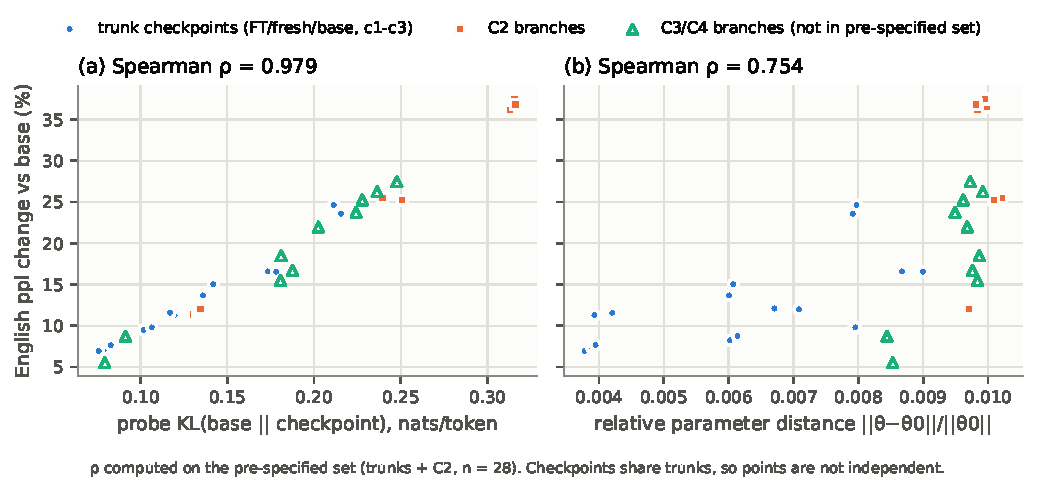
\includegraphics[width=\linewidth]{figures/fig4_p5.pdf}
\caption{English forgetting against (a) probe KL(original $\Vert$ checkpoint) and (b) relative parameter distance, over trunk checkpoints and branches. Spearman $\rho$ is computed on the pre-specified set (trunks and C2 branches); C3/C4 branches (open markers) are shown for reference. Points share trunks and are not independent.}
\label{fig:4}
\end{figure}


Across the pre-specified set of checkpoints (all trunk checkpoints and C2 branches, n = 28), English forgetting was strongly associated with probe KL to the original model (Spearman ρ = 0.979) and less strongly with relative parameter distance (ρ = 0.754) \textbf{[pre-specified descriptive comparison, P5]} (Fig. 4). Adding the C3 branches gives 0.985 vs 0.763 (n = 34) \textbf{[exploratory]}. The checkpoints are not independent: they share trunks and branch starts. The probe blocks are part of the English Wikipedia evaluation set (50 of its 400 blocks), so probe KL and Wikipedia perplexity partly share data. The association with probe KL was also high in the domains that do not overlap the probe (books ρ = 0.962, web ρ = 0.966; Wikipedia ρ = 0.997) \textbf{[exploratory]} (Fig. 4). Associations between a KL divergence and forgetting have also been reported in post-training: \citet[\emph{Retaining by Doing}, App.~A.5]{chen2026retaining} report a Pearson correlation of 0.52 between KL and forgetting, and RL's Razor \citep{shenfeld2025} relates forgetting to the KL divergence from the base model. Their settings and KL estimates differ from ours, so the values are not directly comparable. This is a comparison of associations, not a causal claim.


\section{Limitations}

\emph{Scale and statistics.} One model (Pythia-410M) from one family. Two trunks (seeds) per condition; practical margins come from two-seed ranges with a 2.0-point floor. ``Meets the practical margin'' means same direction in both pairs plus a mean difference at or above the margin; it is not a significance test, and no correction is made for the many comparisons. The checkpoints in P5 are not independent. The probe for probe KL is drawn from the English Wikipedia evaluation set (50 of 400 blocks), so the P5 association on Wikipedia partly reflects shared data; the books and web sets do not overlap the probe.

\emph{Data and metrics.} The stream is Wikipedia in four languages, about 2.0M tokens per cycle, with training text from 353–407 articles per language (at most 20 blocks each). The contamination rule removed 45\% of candidate held-out blocks for Korean and 60\% for Greek (mostly year and date articles), so the remaining held-out sets are biased toward blocks less similar to training data; absolute values should not be compared across languages. The same 512 tokens carry different amounts of text across languages (Russian about 2.7 times more characters than Korean). Knowledge is measured only by perplexity, which reflects style and distribution more than factual accuracy; the multi-stage study does not use downstream task evaluations. English is measured in three domains only, and PG-19 may overlap Pythia's pre-training data (we interpret changes only). An earlier, separate single-stage phase used a Korean held-out set that shared 32.7\% of its 13-grams with its training data; that set is not used here.

\emph{Design confounds.} In the B trunks, FT trains 120 steps per cycle and fresh 150 (25\% more compute); the B-stage English reversal is confounded by this and was observed post hoc. FT-150 fills replay slots with repeated Greek blocks (25\% more Greek exposure) and does not isolate interference perfectly. The EP arms discard blocks that fail the filter and therefore generate more text than the unfiltered arms (§4); the composition comparison matches the training budget, not the generation cost. In C4, top-p truncation and single-sample noise are confounded; KL matches conditional distributions on sampled prefixes, not the teacher's data distribution; the KL weight equals the NTP weight and was not tuned; KL arms use micro-batch 2 × 16 accumulation versus 4 × 8 for NTP (identical update batches verified); per-component losses were logged only for KL arms. All C2–C4 branches start from the $M_3$ of a fresh trunk; whether the branch results hold from an $M_3$ with a different history (a base-anchor or FT trunk) is untested. H2 (mixing) was not given a pre-specified decision rule. Decision rules were revised before results (gate size criterion, ``same-kind'' practical margins, relaxed C3 monotonicity), with reasons recorded. Post hoc observations (the B-stage reversal, ``base level plus anchor drift'') are not tests.

\emph{Generation and numerics.} Replay is sampled with top-p 0.95, so it follows a truncated distribution and the equality of \citet[Eq.~1]{marek2026} does not hold in our setting. Generation is unconditional from EOS. Base-generated replay in this study contains code (about 13\%) and some degenerate blocks (4-gram repetition ≥ 0.5, about 2\%), and one latest-anchor replay set contains four identical whitespace-only blocks. B-stage generation used batch 48 and C-stage batch 24 with identical code (greedy decoding with and without KV cache matched on 2,048/2,048 tokens; sampling statistics agreed within standard errors). bf16 training is not bit-reproducible. A non-zero numerical floor was observed in the KL implementation, varying with the teacher and replay text (about 0.002–0.021 nats/token). Weights are rounded to fp16 between cycles (same for all conditions), and evaluation is in fp16. Intermittent native process crashes occurred during preparation; affected steps were re-run from scratch by an automatic retry (none occurred during the C3 and C4 runs).


\section{Conclusion}

In multi-stage continual pre-training with self-generated replay, the model that writes the replay determines what is protected. In our runs, an original-model anchor retained English best and English forgetting decreased monotonically with anchor age, while retention of intermediate languages did not follow a simple pattern. Replay from the original model also partially recovered English that had been lost before the branch (9.4–15.7 points below the branch start in every domain and both trunks, not back to the original level). Replaying text sampled from the latest checkpoint with NTP amplified English degradation beyond a budget-matched replay-free control; training on the same text toward the teacher's full distribution removed the detectable excess, identifying hard sampled-target replay as a major contributor. These results come from one 410M model and two trunks per condition. Next steps are an untruncated (top-p 1.0) NTP arm to separate truncation from sampling noise, mixed-anchor KL, the anchor-age curve under KL, larger models, and other streams.

\section*{Code and data availability}

{\sloppy Code, result files, training logs and the paper source are available at \url{https://github.com/DoHyunwooo/replay-anchor-provenance}. All reported experimental metrics are derived from the released result files: per-checkpoint evaluation files, the outputs of the decision-rule scripts (\texttt{c\_check.json}, \texttt{gate\_check.json}), training logs and configurations, and replay metadata. The script \texttt{verify\_draft.py} re-reads or recomputes each experimental number from these files, compares it with the text at the displayed precision, and checks the verdict wording of Table 1; it reports any mismatch and any number it could not check. Some descriptive statistics of the replay text (code share, degenerate and duplicate blocks) and one overlap statistic from the earlier single-stage phase are recomputed by the released scripts from tokenized data; the tokenized data are not redistributed and must be regenerated with the released scripts. Numbers quoted from other papers are taken from those papers.\par}

\section*{Acknowledgments}

The author used AI tools (Claude, Claude Code and ChatGPT) for writing code and drafting the text. All experimental design decisions and all numbers were reviewed by the author, and every experimental number in the paper was checked against the original result files by a script (\texttt{verify\_draft.py}).



\bibliographystyle{plainnat}
\bibliography{references}

\appendix

\section{Hyperparameters}


\begin{table}[t]
\centering
\small
\caption{Hyperparameters of all runs (generated from the code and run configurations by \texttt{hparams.py}).}
\label{tab:3}
\begin{tabularx}{\linewidth}{llX}
\toprule
\textbf{Group} & \textbf{Setting} & \textbf{Value} \\
\midrule
Training & Optimizer & AdamW 8-bit (bitsandbytes, \texttt{adamw\_bnb\_8bit}), re-initialized every cycle \\
Training & Adam β1, β2 & 0.9, 0.999 \\
Training & Adam ε & 1e-8 \\
Training & Weight decay & 0 \\
Training & Gradient clipping (max norm) & 1.0 \\
Training & Learning rate & 1.5e-5, constant after a 10-step linear warmup \\
Training & Precision & fp32 weights with bf16 autocast, gradient checkpointing; weights saved in fp16 after each cycle \\
Training & Batch per update & 32 blocks of 512 tokens (NTP 4 × 8, KL 2 × 16) \\
Training & Steps per cycle & 150 with replay (3,840 new + 960 replay blocks), 120 without (FT) \\
Training & Seeds & 42, 43 (training seed = trunk seed) \\
Generation & Start and stopping & a single EOS token (unconditional); not stopped at EOS \\
Generation & Temperature & 1.0 \\
Generation & Top-p & 0.95 (no top-k; padding ids blocked) \\
Generation & Length & 512 tokens per block \\
Generation & Batch & 48 (B stage), 24 (C stage) \\
Generation & Precision & fp16 weights, KV cache \\
Evaluation & Block length & 512 tokens (511 prediction positions) \\
Evaluation & Held-out blocks & 400 per set (English Wikipedia, PG-19 books, C4 web; Korean, Japanese, Russian, Greek) \\
Evaluation & Probe for probe KL & 50 blocks, every 8th block of the English Wikipedia held-out set \\
Evaluation & Precision & fp16 weights, batch 4 \\
Data & Article cap & 20 blocks (training), 4 blocks (held-out) \\
Data & Contamination rule & drop held-out blocks with more than 10\% of their 13-grams in the training data \\
\bottomrule
\end{tabularx}
\end{table}

\textbf{Logged replay KL in the C4 arms [exploratory].} The replay KL logged during training (mean over logged steps and both trunks) was small: about 0.025 nats/token for the latest teacher, 0.10 for the base teacher.


\end{document}
